\documentclass[10pt]{article}
\usepackage[margin=0.7in]{geometry}
\usepackage[T1]{fontenc}
\usepackage{lmodern}
\usepackage{graphicx}
\usepackage{booktabs,tabularx}
\usepackage[hidelinks]{hyperref}
\setlength{\parindent}{0pt}
\setlength{\parskip}{6pt}
\newcommand{\repo}{https://github.com/aburan28/crypto/blob/codex/envoy-fpga-crypto-pq-20261017/integrations/envoy-fpga-crypto/}
\begin{document}
\begin{center}
{\Large Envoy FPGA crypto: implementation and validation}\\[4pt]
2026-10-18 \quad Run batch: \texttt{envoy-fpga-20261018-rtl-live}
\end{center}

The requested system offloads Envoy's classical and post-quantum operations
to AWS F2. This iteration adds actual hash/arithmetic RTL and checks the
linked Envoy boundary. Full FPGA signature/KEM controllers, mailbox and F2
shell integration, and physical deployment remain unfinished. No CPU/FPGA
speedup or algorithm runtime is measured.

\begin{center}
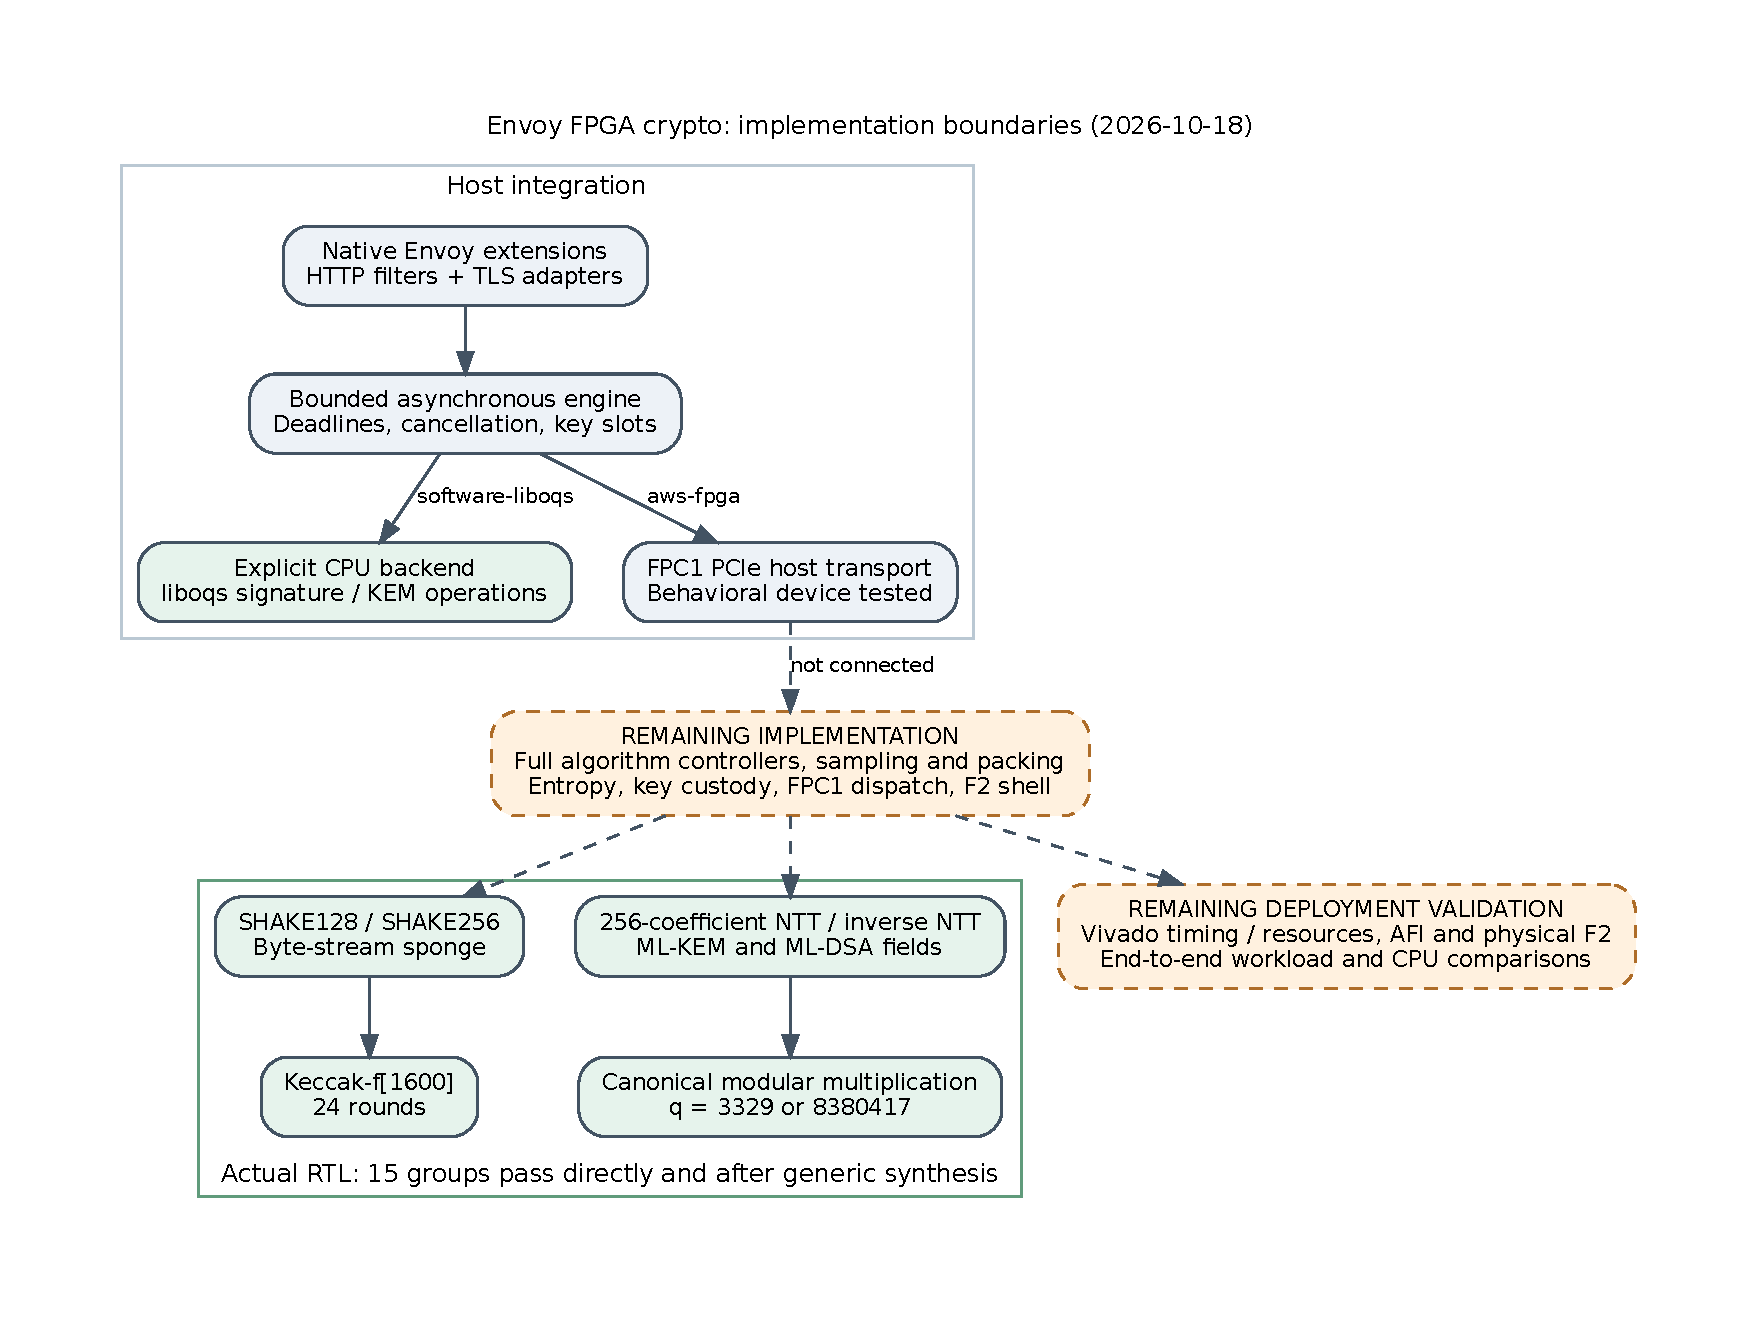
\includegraphics[width=0.94\textwidth,height=0.61\textheight,keepaspectratio]{architecture.pdf}
\end{center}
\textbf{Figure 1.} Solid connections are implemented; dashed connections
require implementation or deployment validation. Functional test groups
are not performance samples, so this explanatory diagram replaces a timing
comparison. Source: \texttt{architecture.dot} in this report's directory.

\textbf{Source identity.} Extends commit
\texttt{3c81607c87c4b896e78a49eb6b7f252c0131a96e},
\href{https://github.com/aburan28/crypto/pull/2122}{PR \#2122}.
Final project hashes and aggregate outcomes are in
\href{\repo docs/receipts/2026-10-18/manifest.json}{the Oct 18 receipt manifest}.
The owner-approved
\href{\repo docs/receipts/2026-10-18/runs.tar.xz}{raw archive} and
\href{\repo docs/receipts/2026-10-18/run-manifest.json}{detailed run manifest}
preserve the original validation batch. The detailed manifest identifies the
execution-era snapshot; the summary includes later documentation/PDF updates.

\section*{Evidence and reproduction}
\href{\repo docs/validation.md}{Validation commands and exact test scope};
\href{\repo docs/rtl-kernels.md}{RTL interface contracts and FIPS 202/203/204 references};
\href{\repo docs/receipts/2026-10-18/README.md}{Oct 18 receipt archive};
\href{\repo docs/reports/2026-10-18/README.md}{full source-linked report}.
The report and diagram are generated with Graphviz and pdfLaTeX; their
editable sources are committed together.
\newpage

\section*{Observed correctness results}
\begin{tabularx}{\textwidth}{@{}lX@{}}
\toprule
Check & Observed result and scope \\
\midrule
Source RTL & Fatal Verilator lint passed; 15/15 native C++ groups passed. \\
Generic synthesis & Structural checks passed; zero combinational loops;
no runtime divider, modulo or latch cells. \\
Generated Verilog & Same 15/15 external groups passed; not a formal
equivalence proof or 30 independent test specifications. \\
Host regressions & 36/36 core, classical TLS, PQ and PQ TLS groups passed again. \\
Linked Envoy & Minimal Envoy v1.39.3 executable linked with the extension. \\
Live HTTP & 5/5 groups passed using CPU liboqs: ML-DSA-65, ML-KEM-768,
independent BoringSSL checks, contexts/256 KiB input, rejection and erasure. \\
Workflow lint & Local actionlint 1.7.7 passed; optional linked Envoy and
BoringSSL/liboqs tests are excluded from this scoped CI job. \\
Root Rust gate & Failed before tests: 26 compilation errors in unchanged
base sources, including duplicate \texttt{Fp4} variants. \\
\bottomrule
\end{tabularx}

Source simulation enables assertions and randomized register initialization.
Public fixture seed: \texttt{0x4650433252544c}. SHAKE is checked against
OpenSSL; NTT is checked against direct evaluation/interpolation and
schoolbook negacyclic convolution. The test's pointwise/base multiplication
is C++ oracle code, not a hardware command. Cancellation, invalid operands,
backpressure, erasure and concurrent independent engines are exercised.

The generic hierarchy has 14,953 coarse cells, not Xilinx utilization.
Writable arrays became registers. This establishes no frequency, physical
DSP/BRAM mapping, power, masking, fault resistance or side-channel result.

\section*{Failures, environment and remaining scope}
The original object-only Envoy check missed a runtime registration collision:
both HTTP factories returned generic \texttt{google.protobuf.Struct}.
Distinct \texttt{FpgaHttp} and \texttt{PqHttp} configurations now give the
factories unique types. Compilation alone did not establish startup.
Successful linked-process startup now exercises both registrations.

The first HTTP run passed 2/5 groups because the harness incorrectly required
content type on empty acknowledgments. Envoy removes that header. Correcting
the harness gave 5/5 without changing the production filter. Nonempty content
types, status, body, cache control and backend labels remain checked.

Intermediate attempts failed on width/unused-signal lint, vendor C++ warning
settings, generated netlist warnings, one script edited during execution,
and an oversized generated model killed during compilation. Logs are retained.
The final flow copies its script and uses byte-addressed SHAKE storage; both
RTL representations pass. Failed attempts used intermediate sources rather
than the final source hash set. Intermediate snapshots and exact initial
standalone lint commands were not frozen; final sources and commands are recorded.

Linux x86-64 shared workspace: four CPU quota cores, 16 GiB memory ceiling;
GCC 14.2.0, Verilator 5.032, sv2v 0.0.13, Yosys 0.52.
There is no isolated benchmark, Vivado, attached F2 or AWS identity.
Build diagnostics are not cryptographic performance measurements.

Complete ML-KEM/ML-DSA controllers, sampling, packing, hardware polynomial
products, entropy, key custody and FPC1 dispatch remain. Classical hardware
cores, an AFI, final FN-DSA and comprehensive FPGA scheme coverage are absent.
Stateful LMS/XMSS are also absent. The 262-mode liboqs catalog is an explicit CPU backend. Oct 17 exhaustive
catalog and sanitizer results are historical and were not rerun in this batch.
TLS KEM key shares remain BoringSSL CPU work; the private-key signing callback
does not offload them.
Actual Envoy TLS/F2 listeners and the default full extension selection were
not tested; live HTTP used ephemeral loopback ports and an explicit CPU backend.

The index-calculus scoreboards, timeline, curve diagrams and performance
charts remain unchanged: this change yields no corresponding curve/ECDLP
finding or performance measurement.

\end{document}
